% Imports and Packages
\documentclass[titlepage,12pt]{article}
\usepackage{biblatex} % Bibliography
\usepackage{graphicx} % Required for inserting images
\usepackage{caption}
\usepackage[margin=1in]{geometry}
\usepackage{amsmath, amssymb, amsthm}
\usepackage{mathtools}


% Title stuff
\title{Optimal Play and Human Behavior in the Showcase Showdown}
\author{Arjun Subramanian, Ethan Geppel, Owen Smith}
\date{January 2026}

% Include other files
\addbibresource{bibliography.bib}
\graphicspath{ {./plots/} }


% Beginning of document
\begin{document}

% Create title page
\maketitle


% Create table of contests page
\tableofcontents
\newpage

\section{Abstract}
The Showcase Showdown from The Price Is Right is a sequential decision problem in which contestants must choose whether to stop or continue under uncertainty. We model the game using dynamic programming and validate the resulting strategies with large-scale Monte Carlo simulations and a newly compiled dataset of over 11,000 Showcase Showdown games.

By comparing theoretically optimal strategies with simulated play and observed contestant behavior, we quantify systematic deviations in win probabilities and decision quality. While optimal play favors later contestants, empirical outcomes reveal consistent departures from optimal behavior, especially in high-information decision states. These patterns are well explained by bounded rationality: later contestants benefit from small increases in decision precision, whereas earlier contestants require substantially higher rationality to realize strategic advantages.

Overall, this work combines theory, simulation, and real-world data to provide insight into sequential decision-making and human behavior under risk.

\section{Introduction}

\subsection{The Showcase Showdown Description and Formalization}

\emph{The Price Is Right}, originally hosted by Bob Barker and first airing on September 4, 1972, is one of the longest-running and most recognizable game shows in American television history. Among its various pricing games, the \emph{Showcase Showdown} serves as the decisive contest determining which contestant advances to the final showcase round. Despite its apparent simplicity, the Showcase Showdown embodies a rich sequential decision-making problem under uncertainty, making it a natural subject for probabilistic and game-theoretic analysis.

The Showcase Showdown is played by three contestants, denoted Contestant~1 (C1), Contestant~2 (C2), and Contestant~3 (C3), who act sequentially in that order. Each contestant spins a large wheel divided into twenty equally sized segments labeled
\[
\{5, 10, 15, \dots, 100\} \text{ cents},
\]
with each outcome occurring with equal probability. Contestants accumulate points by spinning the wheel, subject to a strict upper bound of $100$ cents.

Each contestant must take exactly one spin on their turn. After observing the outcome of their first spin, a contestant may choose either to \emph{stand} or to \emph{spin again}. If a second spin is taken, its value is added to the first. If the resulting total exceeds $100$, the contestant \emph{busts}, receiving a score of zero and losing against all non-bust scores. A contestant who spins exactly $100$ on their first spin is not permitted to spin again. Contestants observe the final totals of all players who act before them, but have no information about future spins beyond the known distribution of wheel outcomes.

At the conclusion of play, the contestant with the highest total not exceeding $100$ wins the Showcase Showdown. In the event of a tie for the highest non-bust score, the tied contestants participate in a symmetric spin-off to determine the winner where each participant spins the wheel only once \cite{ShowcaseShowdownWiki}.

We now formalize the Showcase Showdown as a finite, stochastic, sequential game. Let the set of possible wheel outcomes be
\[
\Omega = \{5, 10, 15, \dots, 100\},
\]
with each outcome occurring with probability $1/20$. For contestant $i \in \{1,2,3\}$, let $X_i \in \Omega$ denote the outcome of the first spin and $Y_i \in \Omega$ denote the outcome of the second spin, if taken. The total score of contestant $i$ is given by
\[
S_i =
\begin{cases}
X_i, & \text{if the contestant stands after one spin}, \\
X_i + Y_i, & \text{if } X_i + Y_i \le 100, \\
0, & \text{if } X_i + Y_i > 100.
\end{cases}
\]

After observing $X_i$, contestant $i$ chooses an action
\[
a_i \in \{0,1\},
\]
where $a_i = 0$ corresponds to standing and $a_i = 1$ corresponds to spinning again. The action $a_i = 1$ is infeasible if $X_i = 100$, and the initial spin is mandatory for all contestants. The information set of contestant $i$ consists of the realized totals $\{S_1, \dots, S_{i-1}\}$ of earlier contestants and their own first-spin outcome $X_i$.

\subsection{Historical Context}

The Price Is Right’s Showcase Showdown  has long attracted attention from probabilists and game theorists as a simple yet high-stakes sequential game. Early analyses derived the optimal stopping rules under idealized assumptions. For example, Coe and Butterworth (1995) formulated the one-player stopping problem for the wheel and identified the optimal threshold strategy \cite{Coe1995}. Sakaguchi (2005, 2007) extended this to two-player settings, deriving equilibrium stopping rules under different scoring formats and information structures \cite{Sakaguchi2005,Sakaguchi2007}. More recently, Mazalov and Ivashko (2010) considered the general $n$-player version of this game. They modeled each player observing the cumulative sum of independent $\mathrm{Unif}[0,1]$ draws (scaled versions of the wheel outcomes) and stopping optimally. Using dynamic programming, they explicitly solved for the subgame-perfect equilibrium strategy in the general sequential game \cite{Mazalov2010}. Similarly, Bayón et al.\ (2025) analyze variants of the wheel game with “unlimited” spins and various information rules, obtaining the corresponding Nash equilibrium strategies \cite{Bayon2025}.

Parallel to these theoretical studies, empirical and experimental work has tested actual contestant behavior. Tenorio and Cason’s influential “To Spin or Not to Spin?” (2002) paper derives the unique subgame-perfect equilibrium for The Wheel and then compares it against data from the televised game show and lab experiments. They find that contestants often deviate from the optimal stopping rule when the decision is difficult, in ways consistent with omission/commission biases. In other words, real players sometimes act too conservatively or aggressively relative to the equilibrium benchmark. These departures proved largely insensitive to the monetary stakes of the game. In related work, Klein Teeselink et al.\ (2024) use forty years of Showcase Showdown data to show systematic failures of backward induction: contestants tend to simplify the game and focus on beating the next player rather than optimizing the full sequential game. They model this behavior with a quantal-response framework that allows for limited foresight \cite{Teeselink2024}. Overall, these prior studies establish both the theoretical solution of the Showcase Showdown and the fact that real contestants often violate it in predictable ways \cite{ChatGPT2026}.

\subsection{Purpose and Overview of This Paper}

In this paper, we build on the above literature by directly comparing actual contestant play to theoretical benchmarks. Using a new dynamic programming model, we compute the equilibrium stopping thresholds that a perfectly rational player \emph{should} use at each decision point in the Showcase Showdown. Leveraging a large empirical dataset—consistent with and extending prior work—containing over 6{,}000 episodes and more than 10{,}000 Showcase Showdown games, we then analyze how frequently real contestants follow these theoretically optimal strategies. The central goal of this study is to analyze both the magnitude and structure of deviations between optimal play and observed behavior, and to explain these deviations through the lens of bounded rationality.

Methodologically, the paper proceeds in three stages. First, we compile empirical data from the game show itself, examining win probabilities, stopping behavior, and decision accuracy across different game states and contestant positions. Second, we formally solve the Showcase Showdown using dynamic programming and game-theoretic tools, deriving subgame-perfect equilibrium strategies for each contestant position under full rationality. These results serve as the theoretical benchmark. Lastly, we validate the analytical results using large-scale Monte Carlo simulations, which allow us to verify equilibrium predictions, isolate the effects of information and turn order, and evaluate the robustness of the optimal strategies under repeated play.

Beyond measuring optimality gaps, this paper also explores how strategic behavior changes under alternative assumptions. We analyze how much skill matters for each contestant by comparing empirical win rates to those predicted by optimal and random strategies. We also introduce a bounded-rationality framework—specifically a quantal response model—to study how imperfect decision-making affects outcomes. By estimating rationality parameters from observed behavior, we assess how closely real contestants resemble theoretically rational agents.

Taken together, this paper aims to provide a comprehensive comparison between how contestants \emph{should} play and how they \emph{actually} play, combining theory, simulation, and real-world data. In doing so, it contributes both a methodological framework for analyzing sequential stopping games and new empirical insights into human decision-making under risk and strategic uncertainty.

\section{Research}

\subsection{Empirical Data}

The empirical analysis in this paper is based on Showcase Showdown records scraped from publicly available episode summaries hosted on the \emph{The Price Is Right Episode Guide} website (\texttt{https://tpirepguide.com}) \cite{tpirepguide}. Episode pages were traversed programmatically, and the written descriptions of each Showcase Showdown were extracted along with basic episode metadata such as episode identifiers and air dates.

After cleaning and validation, the final dataset consists of 6{,}175 episodes, representing 11{,}215 individual Showcase Showdown instances. Each instance corresponds to a single main-round Showcase Showdown with exactly three contestants acting in fixed order: Contestant~1 (C1), Contestant~2 (C2), and Contestant~3 (C3). Wheel outcomes were normalized to integer values in cents and restricted to the set $\{5,10,15,\ldots,100\}$ to ensure consistency across eras.

The analysis focuses exclusively on the main-round spin-or-stay decision. Contestants were required to have either one spin (stand) or two spins (spin again), and any spins arising from tie-break procedures or bonus events were excluded from the decision variable. Records containing invalid spin values, inconsistent totals, or incomplete contestant information were removed rather than repaired, resulting in a dataset that is structurally consistent with the assumptions of the theoretical and simulation models developed later in the paper. Here is the overall win rate of each player.

\begin{figure}[htbp]
    \centering
    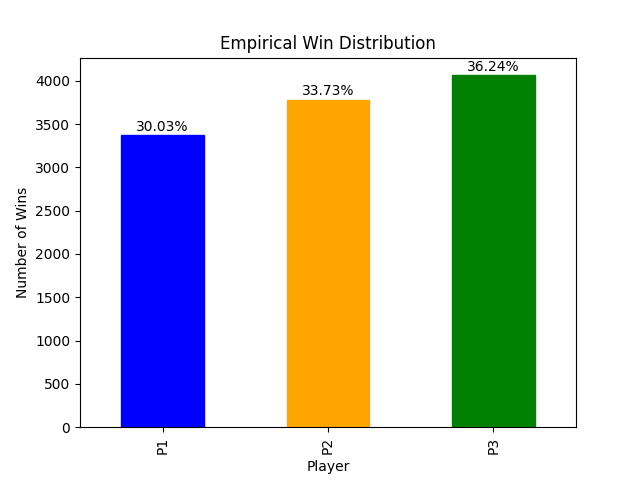
\includegraphics[width=0.8\textwidth]{plots/empirical_win_distribution.png}
    \caption{Bar graph of the win distribution of each contestant}
    \label{fig:empirical_winrate}
\end{figure}

As seen in Fig \ref{fig:empirical_winrate} each player wins around 1/3 of the time with subsequent contestants winning more frequently. As demonstrated later in the paper, this is not due to random chance but is actually the expected behavior. 

\begin{figure}[htbp]
    \centering
    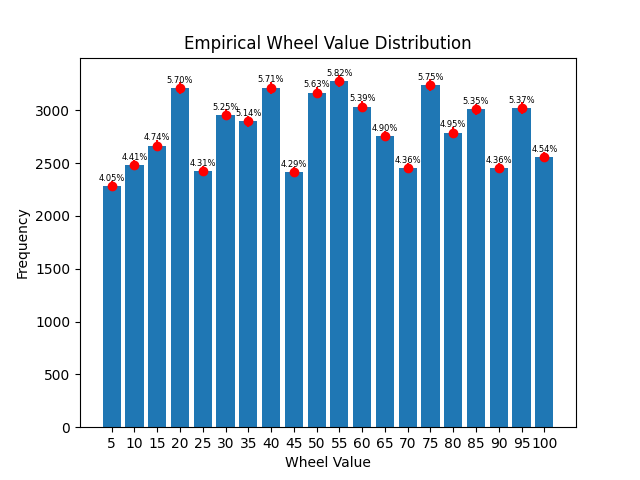
\includegraphics[width=0.8\textwidth]{plots/empirical_wheel_value_distribution.png}
    \caption{Frequency of landing on any given wheel value accumulated over all gathered spins}
    \label{fig:wheel_spins}
\end{figure}

Figure~\ref{fig:wheel_spins} displays the empirical distribution of wheel outcomes across all recorded Showcase Showdown spins in our dataset. The observed frequencies are relatively flat across the twenty possible outcomes, with no value exhibiting a pronounced deviation from the uniform benchmark. This visual evidence is consistent with the findings of Tenorio~\cite{Tenorio2002}, who formally tested the distribution of wheel outcomes using a chi-square goodness-of-fit test and failed to reject the null hypothesis of uniformity. In light of both the prior statistical analysis and the empirical stability observed in our data, we assume throughout the remainder of this paper that each wheel value in $\{5,10,15,\ldots,100\}$ is drawn independently and uniformly at random.

\subsection{Dynamic Programming}

We model the Showcase Showdown as a finite-horizon sequential decision problem with perfect information and stochastic transitions. Each contestant acts exactly once, in fixed order, and faces a binary decision after observing the outcome of their first spin: either \emph{stand} or \emph{spin again}. Wheel outcomes are assumed to be i.i.d.\ and uniformly distributed over the set $\{5,10,\ldots,100\}$, which we normalize to integer values $\{1,2,\ldots,20\}$ for computational convenience.

Let $p_i \in \{0,1,\ldots,20\}$ denote contestant $i$’s final total, where $p_i = 0$ represents a bust. Ties are resolved symmetrically, so win probabilities are fractional when totals coincide. The objective of each contestant is to maximize their probability of winning the Showcase Showdown.

\paragraph{Third Contestant (C3).}
Given fixed totals $(p_1,p_2)$ for the first two contestants and an initial spin outcome $s \in \{1,\ldots,20\}$, the third contestant chooses whether to spin again. Define
\[
V_3(p_1,p_2,s,a) = \Pr(\text{C3 wins} \mid p_1,p_2,s,a),
\]
where $a \in \{0,1\}$ denotes standing or spinning again. If C3 stands ($a=0$), the win probabilities are determined deterministically by comparing $s$ to $\max\{p_1,p_2\}$, with ties split evenly. If C3 spins again ($a=1$), the value function is
\[
V_3(p_1,p_2,s,1)
= \frac{1}{20} \sum_{y=1}^{20} V_3^{\text{term}}\!\left(p_1,p_2, \tilde{s}(s,y)\right),
\]
where $\tilde{s}(s,y)=0$ if $s+y>20$ (bust) and $\tilde{s}(s,y)=s+y$ otherwise, and $V_3^{\text{term}}$ denotes the terminal win probability given final totals. The optimal third-player policy is therefore
\[
\pi_3^\star(p_1,p_2,s)
= \arg\max_{a\in\{0,1\}} V_3(p_1,p_2,s,a).
\]

\paragraph{Second Contestant (C2).}
The second contestant observes $p_1$ and their own first spin $s$. Their value function depends on the expected continuation value induced by the third contestant’s policy:
\[
V_2(p_1,s,a)
= \mathbb{E}_{p_3 \sim \pi_3}\!\left[ \Pr(\text{win} \mid p_1, p_2(a), p_3) \right],
\]
where $p_2(a)=s$ if $a=0$ and $p_2(a)=\tilde{s}(s,Y)$ if $a=1$. Explicitly, for spinning again,
\[
V_2(p_1,s,1)
= \frac{1}{20} \sum_{y=1}^{20}
W\!\left(p_1,\tilde{s}(s,y)\right),
\]
where $W(p_1,p_2)$ is the vector of win probabilities obtained by integrating over C3’s first spin and C3’s policy $\pi_3$. The optimal second-player policy satisfies
\[
\pi_2^\star(p_1,s)
= \arg\max_{a\in\{0,1\}} V_2(p_1,s,a).
\]

\paragraph{First Contestant (C1).}
The first contestant observes only their own first spin $s$ and anticipates optimal play by both later contestants. Their value function is
\[
V_1(s,a)
= \mathbb{E}_{p_2,p_3 \sim \pi_2,\pi_3}
\left[ \Pr(\text{win} \mid p_1(a), p_2, p_3) \right],
\]
with
\[
V_1(s,1)
= \frac{1}{20} \sum_{y=1}^{20}
U\!\left(\tilde{s}(s,y)\right),
\]
where $U(p_1)$ denotes the continuation value induced by the second- and third-player policies. The optimal first-player policy is
\[
\pi_1^\star(s)
= \arg\max_{a\in\{0,1\}} V_1(s,a).
\]

\paragraph{Policy Flexibility and Independence.}
While the above Bellman equations define a subgame-perfect Nash equilibrium when each $\pi_i^\star$ is used, the dynamic programming framework is deliberately more general. Any admissible policy $\pi_3$ can be substituted into the third-player stage, which induces well-defined value functions for C2 and C1. Crucially, when evaluating non-optimal or empirical policies, Contestants 1 and 2 are restricted to \emph{non-oracle} behavior: they compute expected values under the assumption that subsequent players act optimally, rather than conditioning on the actual downstream policy being tested. This preserves the information structure of the game and prevents earlier players from exploiting knowledge that would not be available at the time of decision.

This modular structure allows us to compute win probabilities under optimal play, empirical policies, random strategies, and boundedly rational decision rules within a unified dynamic programming framework.

\subsection{Monte Carlo Simulation}

To validate the dynamic programming results and to assess finite-sample behavior under stochastic play, we additionally implement a large-scale Monte Carlo simulation of the Showcase Showdown. The simulation directly samples random wheel outcomes and simulates full game play according to specified contestant policies. In total, we run $10^7$ independent simulated Showcase Showdowns, which is sufficient to make Monte Carlo estimation error negligible relative to the differences of interest.

Each simulation draw proceeds as follows. Wheel spins are sampled i.i.d.\ from the uniform distribution on $\{5,10,\ldots,100\}$. Contestants act sequentially, and after observing their first spin, each contestant applies a policy $\pi_i$ that maps the observable game state to a binary decision (stand or spin again). Policies may correspond to the optimal dynamic programming solution, empirical strategies, random decision rules, or alternative counterfactual behaviors. Given a policy profile $(\pi_1,\pi_2,\pi_3)$, the simulated outcome of a single game is a random variable
\[
W \in \{1,2,3\},
\]
indicating the winning contestant, with ties resolved according to the official rules.

Formally, for contestant $i$, the Monte Carlo estimate of the win probability is
\[
\hat{p}_i^{\text{MC}} = \frac{1}{N} \sum_{n=1}^{N} \mathbf{1}\{W_n = i\},
\]
where $N=10^7$ and $W_n$ denotes the winner of the $n$th simulated game. By the law of large numbers, $\hat{p}_i^{\text{MC}}$ converges almost surely to the true win probability implied by the policy profile.

The primary role of the Monte Carlo simulation in this paper is validation rather than discovery. Because the dynamic programming formulation computes exact expected win probabilities under the assumed model, agreement between the DP predictions and Monte Carlo estimates provides a strong check on both the mathematical derivation and the implementation. Across all policy profiles examined, the simulated win rates closely match the DP values, confirming that the dynamic programming solution correctly characterizes the probabilistic structure of the game.

\begin{table}[h]
\centering
\caption{Comparison of Dynamic Programming and Monte Carlo Win Rates under Optimal Play}
\label{tab:dp_vs_mc}
\begin{tabular}{lcccc}
\hline
 & \multicolumn{2}{c}{Dynamic Programming} & \multicolumn{2}{c}{Monte Carlo} \\
Contestant & Win Rate (\%) & Win Fraction & Win Rate (\%) & Win Fraction \\
\hline
C1 & 30.82\% & 6311/20480 & 30.82\% & 963/3125 \\
C2 & 32.96\% & 42188819/128000000 & 32.97\% & 3297231/10000000 \\
C3 & 36.22\% & 46367431/128000000 & 36.21\% & 3621169/10000000 \\
\hline
\end{tabular}
\end{table}

As seen in table \ref{tab:dp_vs_mc} the simulation and dynamic programming methods yield similar results.


\section{Applications}

\subsection{Optimal Play}

\begin{figure}[htbp]
    \centering
    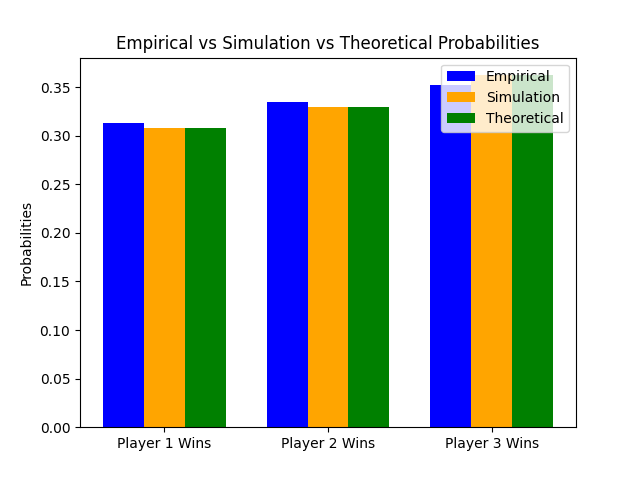
\includegraphics[width=0.8\textwidth]{plots/empirical_simulation_theoretical_comparison.png}
    \caption{Win Probability for each contestant based on Empirical data, Dynamic Programming based optimal strategy, and a Monte Carlo Simulation.}
    \label{fig:compare_winprob}
\end{figure}

Figure~\ref{fig:compare_winprob} compares win probabilities across three settings: empirical contestant behavior, the theoretically optimal strategy computed via dynamic programming, and Monte Carlo simulation under optimal play. As expected, the Monte Carlo estimates closely match the dynamic programming predictions, providing an additional validation that the analytical model correctly captures the probabilistic structure of the game.

A notable deviation arises when comparing these theoretical benchmarks to empirical outcomes. In the data, Contestants~1 and~2 achieve higher win rates than predicted by the optimal model, while Contestant~3 underperforms relative to theory. This pattern suggests that later-stage decision-making is particularly sensitive to strategic precision. Because Contestant~3’s optimal actions are often contingent on narrow payoff differences and require accurate evaluation of future contingencies, even small deviations from optimal play can substantially reduce their win probability. These mistakes effectively transfer winning probability to earlier contestants, inflating their empirical success rates relative to theoretical expectations.

Despite these deviations, Contestant~3 maintains the highest win probability in all three settings. This outcome is consistent with the informational advantage of acting last: Contestant~3 observes the complete set of prior outcomes and can condition their decision on the full game state. 

The dynamic programming results admit a simple and intuitive description of optimal play that can be stated in rule-based terms. Although the underlying model evaluates expected continuation values at every possible state, the resulting equilibrium strategies can be summarized using easily interpretable thresholds that depend on both turn order and available information.

\emph{Contestant 1 (C1).}
Because Contestant~1 acts without information about future spins, their decision reduces to a single cutoff rule. The optimal strategy is to \emph{spin again if and only if} the first-spin total is at most $65$. For totals above $65$, the expected loss from busting outweighs the benefit of improving the score, making it optimal to stand. This threshold reflects the trade-off between increasing one’s own score and the probability of exceeding $100$.

\emph{Contestant 2 (C2).}
Contestant~2 conditions their decision on Contestant~1’s final outcome. If Contestant~2’s initial spin is \emph{less than} Contestant~1’s total, then spinning again is mandatory: standing would guarantee a loss unless Contestant~1 has already busted. If Contestant~2’s initial spin \emph{exceeds} Contestant~1’s total, the strategic problem shifts to anticipating Contestant~3’s response. In this case, Contestant~2 should spin again if their current total is at most $50$, and stand otherwise. This rule reflects the fact that once Contestant~2 is ahead of Contestant~1, the primary risk comes from allowing Contestant~3 an uncontested opportunity to surpass a moderate score.

\emph{Contestant 3 (C3).}
Contestant~3 has complete information about all prior outcomes and therefore follows the most state-dependent strategy. The optimal rule is to spin again whenever their current total is less than the highest non-busted total among Contestants~1 and~2. If either prior contestant has busted, their effective score is treated as zero for comparison. Standing is optimal only when Contestant~3 already holds the lead, as any additional spin would introduce unnecessary bust risk without improving the probability of winning.

Together, these rules illustrate how optimal behavior in the Showcase Showdown depends critically on information structure and turn order. Earlier contestants rely on fixed thresholds, while later contestants employ contingent strategies that respond directly to observed outcomes. These human-readable strategies are used throughout the remainder of the paper to interpret empirical deviations from optimal play and to evaluate alternative behavioral models.

\subsection{Contestant Irrationality}

While the preceding sections assume perfectly rational contestants, empirical evidence demonstrates systematic deviations from optimal play. To model this behavior, we adopt a \emph{bounded rationality} framework using a \emph{quantal response} (QR) specification. In the QR model, the probability that contestant $i$ chooses action $a_i \in \{0,1\}$ (stand or spin again) is an increasing function of the expected payoff difference between actions, tempered by a \emph{rationality parameter} $\lambda \ge 0$. Specifically, the action probability is given by
\[
\Pr(a_i = 1 \mid s_i, \text{state}) 
= \frac{\exp\!\big(\lambda V_i(s_i,1)\big)}{\exp\!\big(\lambda V_i(s_i,0)\big) + \exp\!\big(\lambda V_i(s_i,1)\big)},
\]
where $V_i(s_i,a)$ is the expected win probability from taking action $a$ given first spin $s_i$ and the current game state \cite{Evans2024}.

Intuitively, $\lambda$ controls how strongly a contestant responds to differences in expected payoff. When $\lambda = 0$, choices are completely random, independent of the expected outcomes; as $\lambda \to \infty$, the contestant behaves as a perfectly rational player, deterministically choosing the action that maximizes $V_i(s_i,a)$. In intermediate ranges, contestants probabilistically favor higher-value actions but occasionally make suboptimal decisions, reflecting human decision noise, misperception, or limited computation.

To investigate the impact of bounded rationality on win probabilities, we simulate the Showcase Showdown while varying the $\lambda$ parameter for each contestant. We examine four scenarios:
\begin{enumerate}
    \item Only Contestant~1's rationality is varied; C2 and C3 play optimally.
    \item Only Contestant~2's rationality is varied; C1 and C3 play optimally.
    \item Only Contestant~3's rationality is varied; C1 and C2 play optimally.
    \item All contestants share the same rationality parameter $\lambda$, which is varied simultaneously.
\end{enumerate}

\begin{figure}[htbp]
    \centering
    \begin{minipage}[b]{0.45\textwidth}
        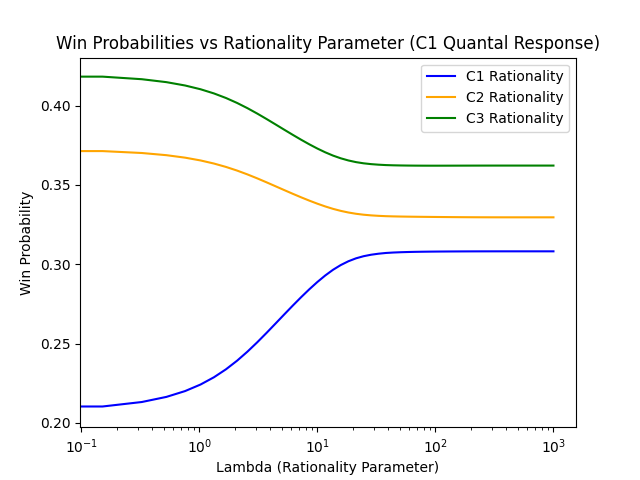
\includegraphics[width=\textwidth]{plots/rationality_C1_quantal_response.png}
        \caption*{(a) C1 rationality varied}
    \end{minipage}
    \hfill
    \begin{minipage}[b]{0.45\textwidth}
        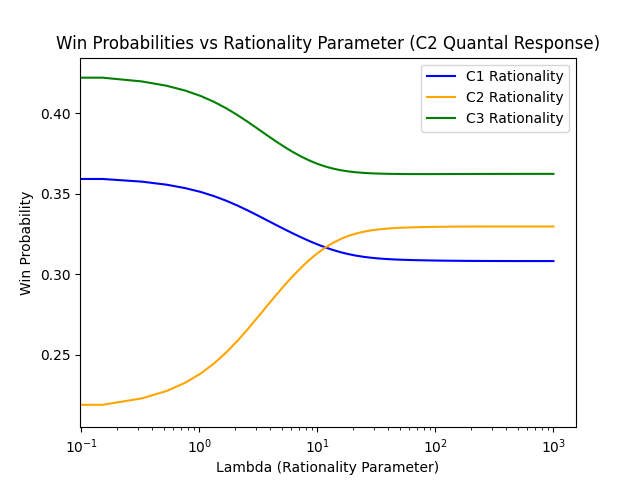
\includegraphics[width=\textwidth]{plots/rationality_C2_quantal_response.png}
        \caption*{(b) C2 rationality varied}
    \end{minipage}

    \vspace{0.5cm}

    \begin{minipage}[b]{0.45\textwidth}
        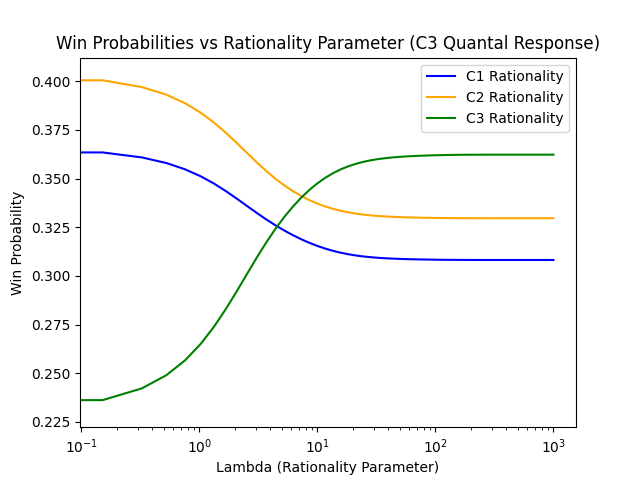
\includegraphics[width=\textwidth]{plots/rationality_C3_quantal_response.png}
        \caption*{(c) C3 rationality varied}
    \end{minipage}
    \hfill
    \begin{minipage}[b]{0.45\textwidth}
        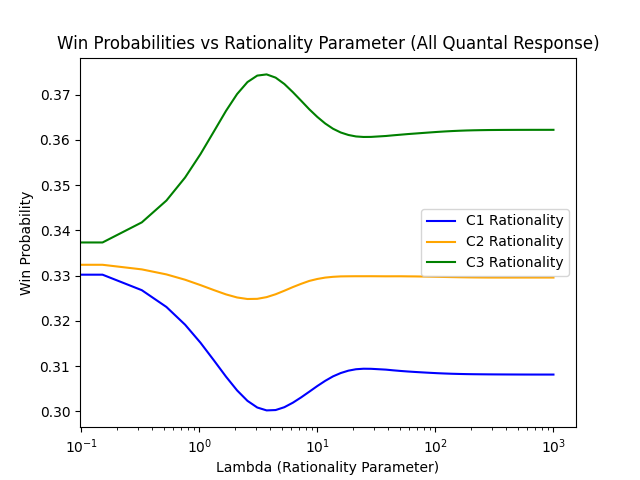
\includegraphics[width=\textwidth]{plots/rationality_all_quantal_response.png}
        \caption*{(d) All contestants vary together}
    \end{minipage}
    \caption{Win probabilities as a function of the rationality parameter $\lambda$. Each subplot varies the rationality of one contestant while holding others fixed, except panel (d) which varies all simultaneously.}
    \label{fig:irrationality_analysis}
\end{figure}

Several key patterns emerge from Figure~\ref{fig:irrationality_analysis}:

\begin{itemize}
    \item \textbf{Initial irrationality:} When contestants are completely irrational ($\lambda = 0$), all win probabilities are approximately equal, around 22.5\%. This high baseline reflects the stochastic advantage of the sequential game even under random play.
    \item \textbf{Rationality tipping points:} As $\lambda$ increases, Contestant~3’s win rate rises sharply first. This is intuitive: C3 often faces “obvious” decisions, such as spinning again when trailing, which have clear expected value advantages. Because these decisions are almost always advantageous, even modest rationality produces a large increase in C3’s wins.
    \item \textbf{Later gains for C1 and C2:} Contestants~1 and~2 see their win probabilities increase only at higher $\lambda$ values (around $\lambda \approx 2$). Their decisions are less immediately decisive because the benefit of spinning again depends on the uncertain subsequent spins of later contestants. Consequently, it requires greater rationality to consistently make choices that improve expected outcomes.
    \item \textbf{Plateauing:} Beyond a certain rationality threshold, further increases in $\lambda$ have minimal effect on the win distribution. Once the key decisions are nearly deterministic, additional rationality does not change outcomes. Notably, the rationality tipping point is largest for C3, reflecting marginal benifit of their decisions while they may seem obvious to a human.
    \item \textbf{Overall distribution dynamics:} As all contestants become more rational simultaneously (panel d), C3 dominates early, but eventually C1 and C2 benefit as they start exploiting spinning opportunities more effectively. This illustrates how information structure and turn order interact with bounded rationality: the earlier a contestant acts, the more rationality is required to realize strategic advantages.
\end{itemize}

\subsection{Applications Beyond \textit{The Price Is Right}}

Although this paper focuses on the Showcase Showdown, the underlying modeling framework extends naturally to a wide range of consumer decision-making problems. In many consumer contexts, individuals face sequential choices under uncertainty and must decide whether to continue searching or to stop and commit to an outcome. Classic examples include price search, product comparison, and timing decisions such as whether to purchase now or wait for future opportunities.

These problems are commonly modeled as optimal stopping or dynamic programming problems. Early work by Stigler \cite{Stigler1961} formalized consumer price search as a trade-off between expected gains from continued search and the costs of acquiring additional information. More recent structural models embed search decisions directly into dynamic choice frameworks, allowing researchers to estimate how consumers optimally—or suboptimally—balance search costs, expected price reductions, and future opportunities \cite{Honka2014,DeLosSantos2012}. The decision to spin again in the Showcase Showdown is formally analogous: contestants must weigh the expected benefit of an additional draw against the risk of busting.

As in the Showcase Showdown, empirical evidence suggests that consumers often deviate from fully optimal strategies. Rather than solving the full dynamic program, individuals frequently rely on heuristics or simplified rules of thumb. Behavioral and marketing research documents the prevalence of satisficing, sequential elimination, and other boundedly rational decision rules in consumer choice \cite{Simon1955,Tversky1972}. These behaviors parallel the quantal response framework used in this paper, in which decision noise interacts with payoff differences to produce systematic deviations from optimal play.

Dynamic models incorporating bounded rationality have proven particularly useful in explaining real-world consumer behavior. For example, Rust \cite{Rust1987} demonstrates how computational costs can rationalize deviations from optimal dynamic decisions, while subsequent work applies similar ideas to loyalty programs, brand choice, and repeat purchasing decisions \cite{Sun2005}. In these settings, consumers face long-run trade-offs whose marginal benefits are often small or uncertain—much like the early-position contestants in the Showcase Showdown—requiring higher levels of rationality to justify optimal actions.

Overall, the methods developed in this paper provide a general framework for analyzing sequential decision-making under uncertainty. By combining dynamic programming with bounded rationality models, the approach offers a flexible tool for studying how real agents make decisions when optimal strategies are complex, payoffs are noisy, and computational resources are limited.


\section{Conclusion}

This paper analyzes decision-making in the Showcase Showdown using dynamic programming, Monte Carlo simulation, and empirical data. We derived subgame-perfect equilibrium strategies for all contestant positions, compared them to over 11{,}000 observed games, and studied the effects of bounded rationality using a quantal response model.  

Compared to prior work, our contributions include a large-scale empirical benchmark, a flexible dynamic programming framework for arbitrary policies, and a quantitative analysis of how deviations from optimal play affect win probabilities. The bounded rationality results reveal tipping points, sequential effects, and nontrivial interactions between contestants’ strategies.  

Limitations include the assumption of uniform wheel outcomes and the exclusion of bonus payments, which have varied over time. Incorporating such incentives would likely increase contestants’ willingness to spin again. Future work could explore bonus effects, risk preferences, learning over repeated plays, and other game complexities.  

Overall, our study provides a unified framework for analyzing sequential stopping games under uncertainty, highlighting both optimal strategies and the systematic ways human behavior diverges from them.


% Prints the used citations from bibliography.bib
\printbibliography

\end{document}